% ----------------------------------------------------------
\chapter{Tecnologia de execução de túneis}
% ----------------------------------------------------------

\section{Métodos de Escavação}

Há diversas formas de se executar túneis, tanto profundos quanto superficiais. Durante a escolha do método de escavação, o engenheiro deve levar em conta diversos fatores, tais como: geometria da seção, comprimento do túnel, condições geológicas, nível da água, restrições quanto às vibrações, estabilidade da cavidade, riscos de assentamentos superficiais, hipóteses de projeto, segurança dos operários, viabilidade ambiental e econômica. Em vista dessa complexidade é possível utilizar mais de um método de escavação ao longo do eixo do túnel. A \autoref{metodos_escavacao} resume os principais métodos de escavação.

\begin{figure}[H]
	\begin{center}
		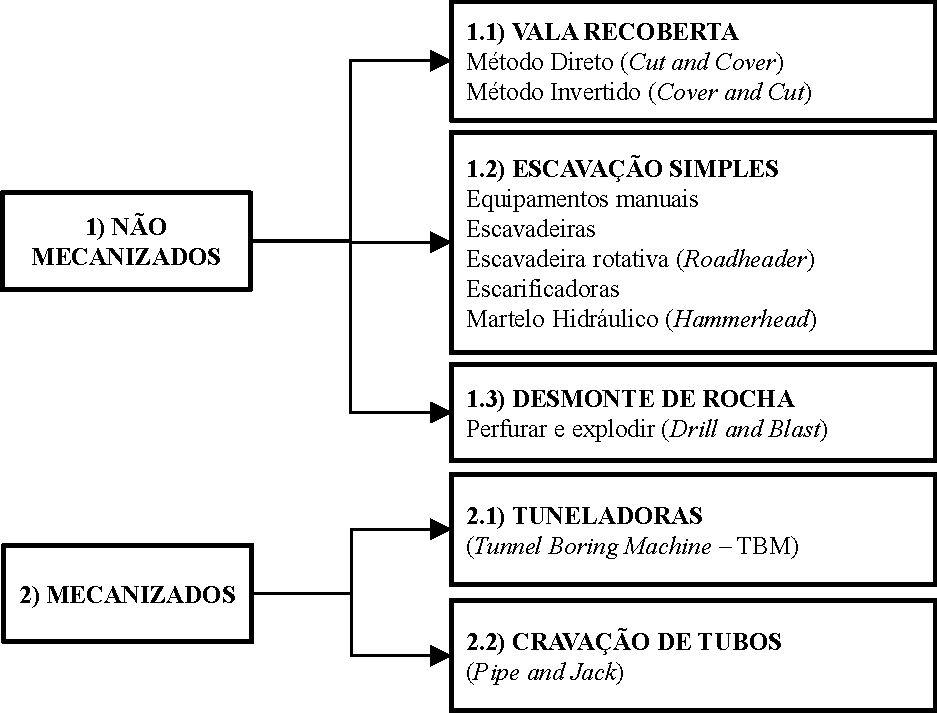
\includegraphics[scale = 1]{0301-métodos de escavação de túneis.pdf}
	\end{center}
	\caption{\label{metodos_escavacao}Métodos de escavação de túneis}
\end{figure}

Os métodos se dividem em dois grandes grupos: 1) não mecanizados (convencionais) e 2) mecanizados. A diferença é que este último é caracterizado pela presença de tuneladoras, que são máquinas especializadas em adentrar a frente de escavação. Os métodos ditos “não mecanizados” não possuem essas máquinas especializadas e podem ser agrupados em: vala recoberta, escavação simples e desmonte de rocha.

\subsection{Vala recoberta}

O método da vala recoberta é utilizado preferencialmente para túneis superficiais. Pode ser executado de duas formas: direta (\textit{Cut and Cover}) ou invertida (\textit{Cover and Cut}). A \autoref{vala_recoberta} e \autoref{etapa_execucao_vala_recoberta} ilustram esse método.

\begin{figure}[H]
	\begin{center}
		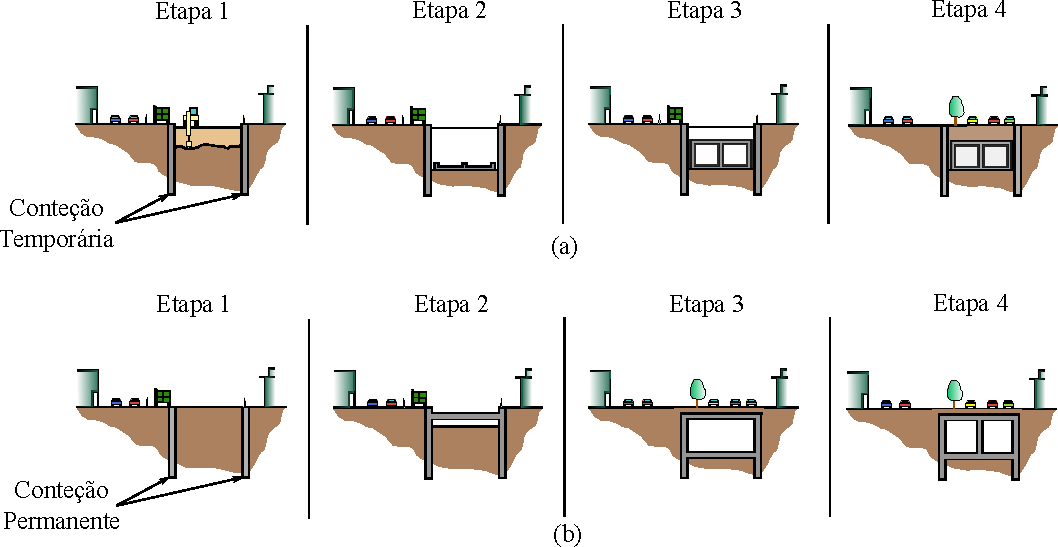
\includegraphics[scale = 0.8]{0302-vala recoberta.pdf}
	\end{center}
	\caption{\label{vala_recoberta}(a) \textit{Cut and Cover} e (b) \textit{Cover and Cut} (adaptado de: \citeonline[p. 5-2]{FederalHighwayAdministration2009})}
\end{figure}

\begin{figure}[H]
	\begin{center}
		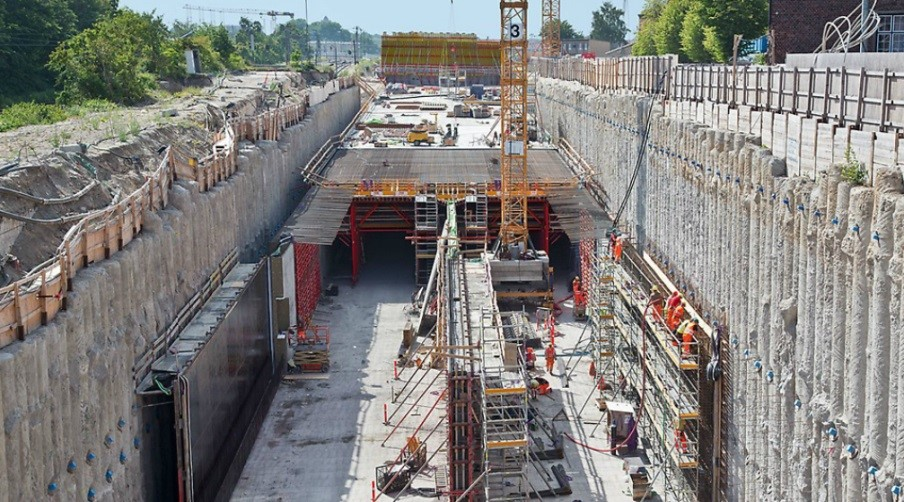
\includegraphics[scale = 1]{0303-etapa de execução pelo método de vala recoberta direta.jpg}
	\end{center}
	\caption{\label{etapa_execucao_vala_recoberta}Etapa de execução pelo método de vala recoberta direta no projeto \textit{Nordhavnsvej}, em Compenhague, Dinamarca (fonte: \citeonline[p. 1]{ROADTRAFFIC-TECHNOLOGY2019})}
\end{figure}

Como o presente trabalho está delimitado aos túneis profundos esse método de escavação estará fora do escopo desta tese. Além disso, o comportamento mecânico desse túnel é diverso daqueles profundos que, tal como será visto no Capítulo 4, mobilizam a resistência do maciço na estabilidade da cavidade.


\subsection{Escavação simples}

A escavação simples é o método que permite maior flexibilidade quanto à geometria da seção e é ideal para escavar galerias de formatos complexos como, por exemplo, estações e conexões. Essa escavação pode ser feita com uma combinação de ferramentas manuais e equipamentos mecânicos, como escavadeira simples, escavadeira rotativa (\textit{Roadheader}), escarificador e martelo hidráulico (\textit{Hammerhead}) (\autoref{escavadeiras}). A produtividade desse método varia, mas dificilmente ultrapassa 10 m/dia de avanço.

\begin{figure}[H]
	\begin{center}
		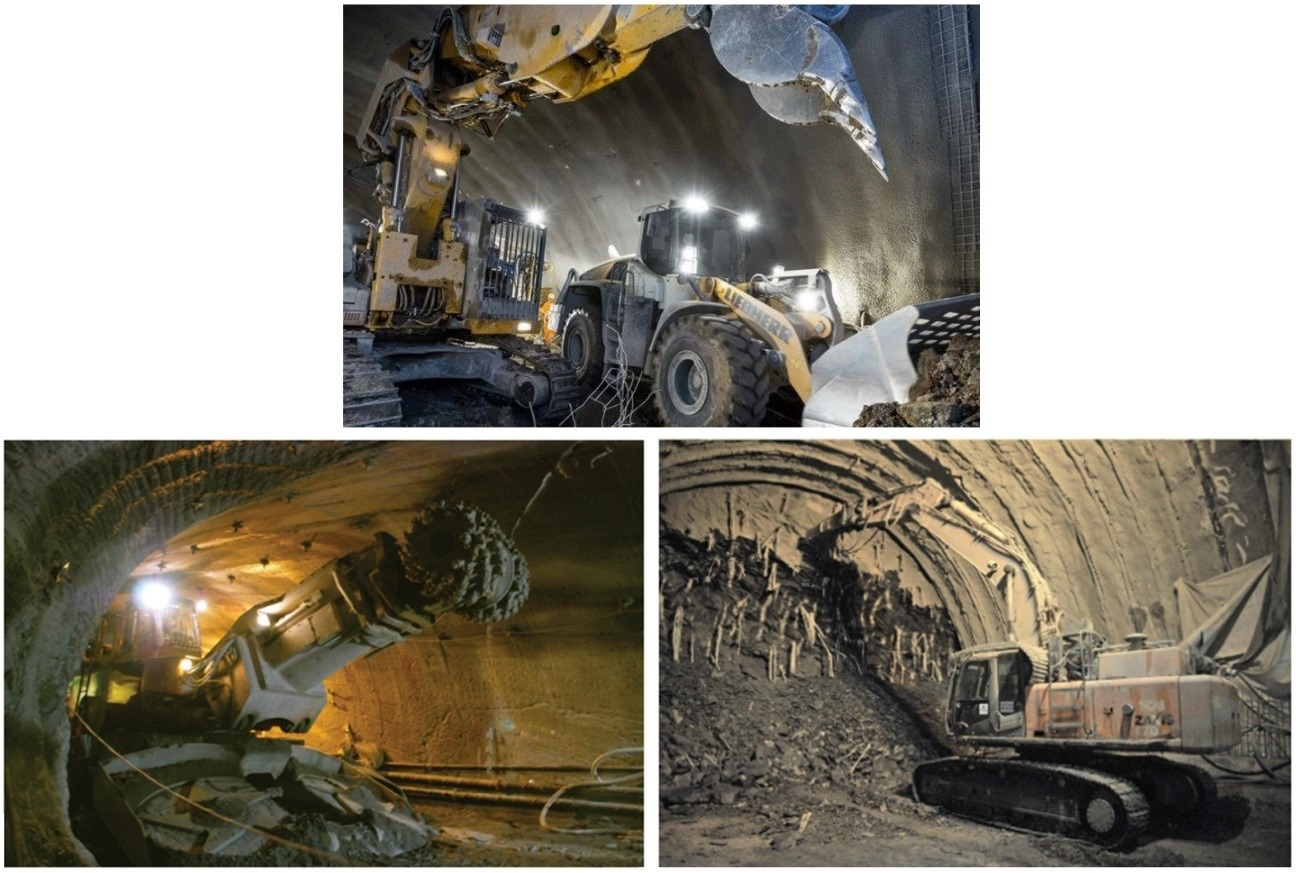
\includegraphics[scale = 1]{0304-escavadeiras,escarificadora,rotativa e martelo hidraulico.jpg}
	\end{center}
	\caption{\label{escavadeiras}Superior à esquerda: escavadeiras (fonte: \citeonline[p. 1]{Pierrat2014}); superior à direita: escarificadora; inferior à esquerda: escavadeira rotativa (fonte: \citeonline[p. 1]{Mitterndorfer2013}) e inferior à direita: martelo hidráulico  (fonte: \citeonline[p. 1]{WORDHIGHWAYS2015})}
\end{figure}


\subsection{Desmonte de rocha}

Quando há dificuldade de penetração no maciço, é necessário utilizar o método de perfuração e detonação, que consiste em perfurar, instalar o material explosivo e detonar a frente de escavação. O ciclo desse método é ilustrado na \autoref{sequencia_detonacao} e \autoref{sequencia_detonacao_fotos}.

\begin{figure}[H]
	\begin{center}
		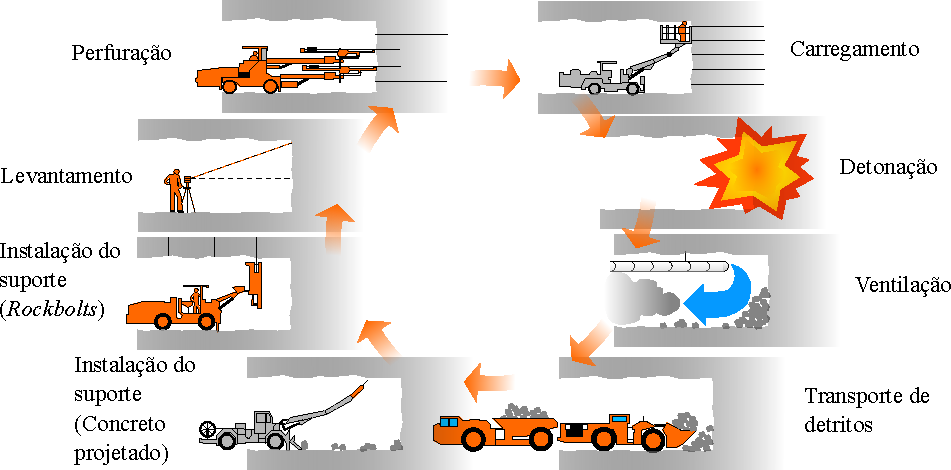
\includegraphics[scale = 1]{0305-sequencia detonação.pdf}
	\end{center}
	\caption{\label{sequencia_detonacao}Sequência executiva do método de construção por desmonte de rocha (adaptado de: \citeonline[p. 215]{Heinio1999})}
\end{figure}

\begin{figure}[H]
	\begin{center}
		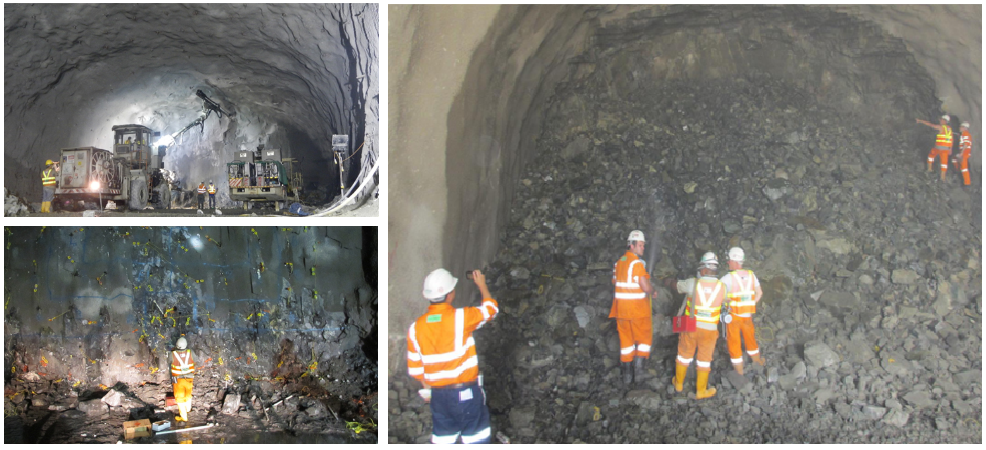
\includegraphics[scale = 0.6]{0306-perfuracao,instalacao das cargas e frente detonada.png}
	\end{center}
	\caption{\label{sequencia_detonacao_fotos}Superior à esquerda: perfuração; inferior à esquerda: instalação das cargas; à direita: frente de escavação após detonação (fonte: \citeonline[p. 1]{Grad2013})}
\end{figure}

\subsection{Tuneladora}

As tuneladoras, tal como ilustrada na \autoref{representacao_tuneladora}, nada mais são do que a evolução do método de escavação com plataformas de Marc Brunel desenvolvido em 1843 (durante a construção do túnel subfluvial sob o rio Tâmisa em Londres). Atualmente, esse tipo de escavação é totalmente mecanizada e possui excelente regularidade da superfície escavada. A produtividade depende de vários fatores (diâmetro da seção do túnel, condições do maciço, potência e tamanho da máquina, tipo de revestimento e experiência das equipes) e pode atingir até 20m/dia \cite[p. 98]{Brox2017}. Geralmente possuem maquinário acoplado para executar o revestimento em concreto projetado ou pré-moldado. Quando o maciço a ser escavado é pouco resistente utiliza-se um escudo (\textit{Shield}) ou lama sob pressão imediatamente anterior à frente de escavação para evitar o colapso da cavidade. As principais desvantagens são os custos e a dificuldade de transporte da máquina.

\begin{figure}[H]
	\begin{center}
		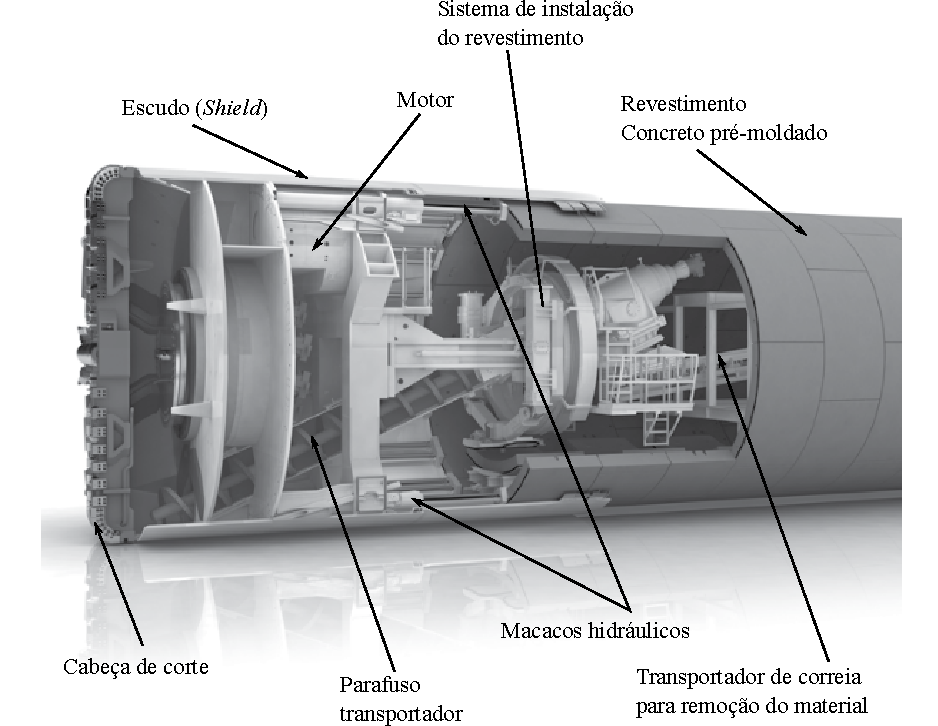
\includegraphics[scale = 1]{0307-representacao 3D de uma tuneladora.pdf}
	\end{center}
	\caption{\label{representacao_tuneladora}Representação 3D de uma tuneladora (adaptado de: \citeonline[p. 151]{Chapman2018})}
\end{figure}

\subsection{Cravação de tubos}

Por fim, o método mecanizado de cravação de tubos consiste em conectar dois poços cravando tubos com auxílio de macacos hidráulicos, uma parede de reação e uma pequena tuneladora (com ou sem escudo). Esse método é comum quando se tem poucas distâncias a vencer, túneis superficiais e solos brandos. São, portanto, preferencialmente utilizados em obras de fornecimento de água, esgoto, eletricidade e gás nos centros urbanos. A \autoref{cravacao_tubos} e \autoref{cravacao_tubos_fotos} ilustram esse método de escavação.

\begin{figure}[H]
	\begin{center}
		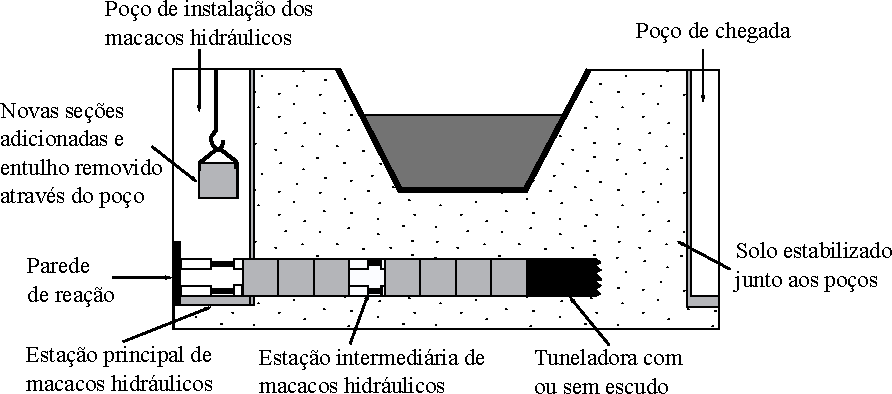
\includegraphics[scale = 1]{0308-metodo de cravacao de tubos.pdf}
	\end{center}
	\caption{\label{cravacao_tubos}Ilustração do método de cravação de tubos sob um canal (adaptado de: \citeonline[p. 227]{Chapman2018})}
\end{figure}

\begin{figure}[H]
	\begin{center}
		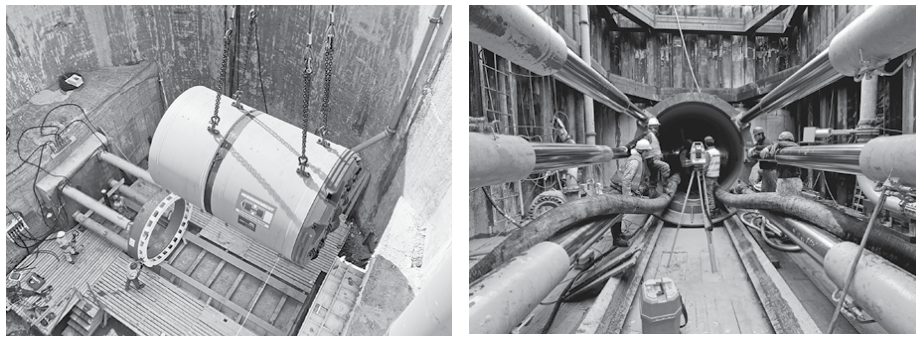
\includegraphics[scale = 0.6]{0309-poco de macacos hidraulicos com a descida da TBM.png}
	\end{center}
	\caption{\label{cravacao_tubos_fotos}À esquerda: vista de cima de um poço de macacos hidráulicos com a descida da TBM; à direita: vista frontal do túnel (fonte: \citeonline[p. 227]{Chapman2018})}
\end{figure}

Como este trabalho está delimitado aos túneis profundos, esse método de escavação estará fora do escopo dessa tese. Apesar de mobilizar a resistência do maciço possuí condições de contorno bem diversas de túneis profundos.

\section{Pré-suportes e melhoramento do maciço}

O termo \textbf{pré-suporte} não compreende apenas os elementos físicos, mas também técnicas que são utilizadas visando à estabilidade do maciço antes de iniciar a etapa de escavação da face de avanço do túnel. São comumente empregados em maciços ou regiões do maciço que apresentam riscos de desabamentos iminentes (\autoref{simulacao_falha}).

\begin{figure}[H]
	\begin{center}
		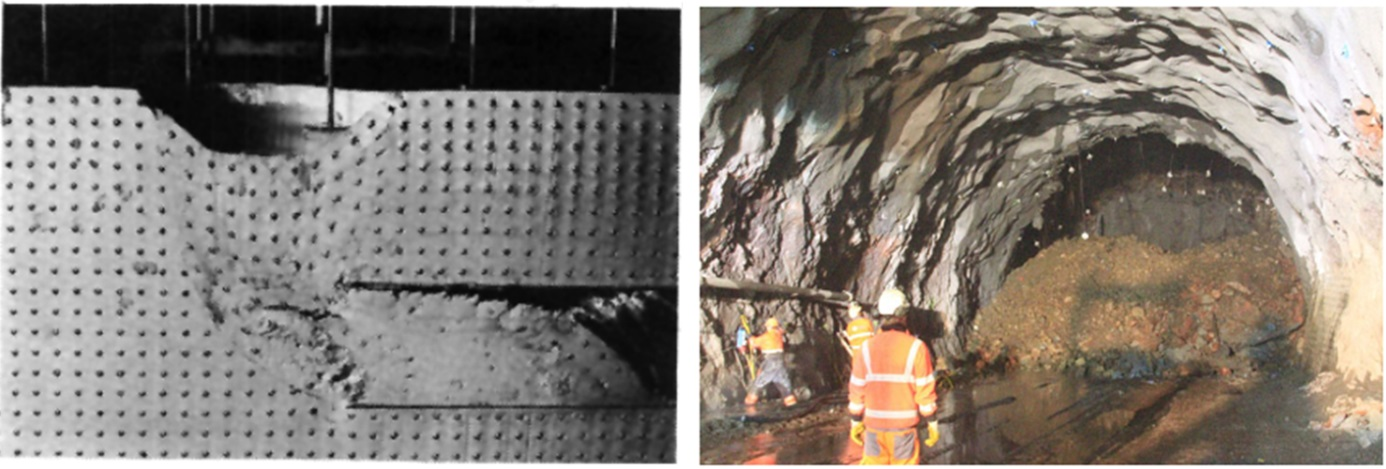
\includegraphics[scale = 1]{0310-simulacao da falha na face de um tunel e colapso progressivo da face.png}
	\end{center}
	\caption{\label{simulacao_falha}À esquerda, simulação da falha na face de um túnel (fonte: \citeonline[p. 245]{Schofield1980}); à direita, o colapso progressivo da face do túnel rodoviário \textit{Vadlaheidi} na Islândia (fonte: \citeonline[p. 1]{Reynolds2015})}
\end{figure}

Alguns exemplos de técnicas de pré-suporte são:

\begin{alineas}
	
	\item \textbf{enfilagens}: instalação de barras, placas ou perfis de aço no interior do maciço, logo acima do perímetro da seção de escavação;
	
	\item \textbf{escavação parcializada}: criação de taludes ou nichos de escavação sustentados com concreto projetado;
	
	\item \textbf{tirantes frontais}: consiste na instalação de tirantes de fibra de vidro ou injeções de concreto na face de escavação. Comumente utilizados quando o túnel tem que passar por zonas instáveis como, por exemplo, falhas geológicas;
	
	\item \textbf{pré-confinamento com ar comprimido}: consiste em aplicar ar com uma determinada pressão no interior da galeria de escavação. Essa técnica é comum em solos moles ou saturados com água;

	\item \textbf{técnicas de melhoramento}: injeção de nata de cimento sobre pressão (\textit{Jet Grouting}) ou consolidação do solo por meio do congelamento com nitrogênio líquido (ou com salmoura), injeções químicas, ou ainda, rebaixamento do lençol freático.

\end{alineas}

Mais detalhes sobre essas técnicas podem ser encontradas em  \citeonline[p. 9-36]{FederalHighwayAdministration2009}, \citeonline[p. 21]{Maidl2013} e em \citeonline[p. 77]{Chapman2018}. Como neste trabalho estamos interessados na modelagem da lei constitutiva do maciço não foram consideradas essas técnicas de pré-suporte na modelagem.

\section{Revestimento de túneis}

O revestimento de um túnel (também conhecido como suporte) tem como finalidade atender critérios operacionais de manutenção e de estabilidade da cavidade a curto, médio e longo prazo quando o maciço por conta própria não atende esses critérios. O revestimento é composto por um \textbf{revestimento primário} e, quando necessário, um \textbf{revestimento secundário}. A \autoref{secao_tunel_rodoviario} ilustra os elementos de uma seção típica de um túnel rodoviário.

\begin{figure}[H]
	\begin{center}
		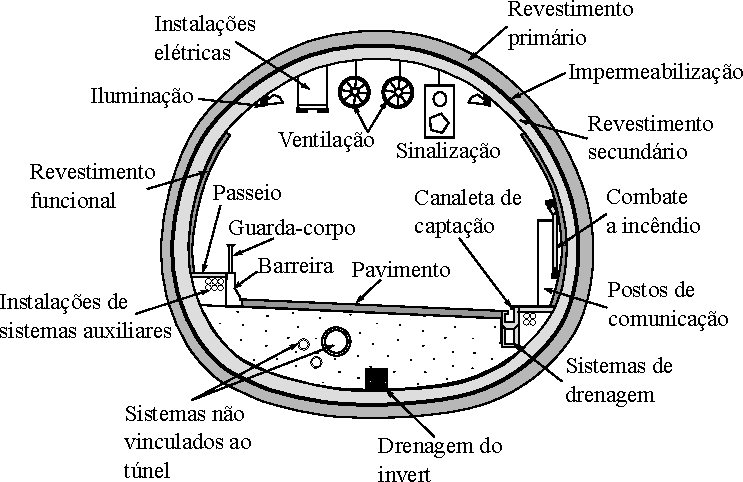
\includegraphics[scale = 1]{0311-ilustracao do revestimento e elementos internos de um tunel rodoviario.pdf}
	\end{center}
	\caption{\label{secao_tunel_rodoviario}Ilustração do revestimento e elementos internos de um túnel rodoviário (adaptado de: \citeonline[p. 20]{DEPARTAMENTODEESTRADASERODAGEMSAOPAULO2005})}
\end{figure}

O \textbf{revestimento primário} compreende os elementos físicos de suporte inicial (aplicados imediatamente após a escavação), com a finalidade de manter a cavidade do túnel estável. Contudo, quando os elementos de suporte inicial não são suficientes para estabilização da cavidade no médio e longo prazo, adicionam-se mais elementos constituindo assim o \textbf{revestimento secundário}. Quando se utiliza o revestimento secundário, o revestimento primário é comumente projetado com a finalidade exclusiva de garantir a estabilidade local da cavidade do túnel durante o período construtivo. Contudo, ambos contribuem para a estabilidade de médio e longo prazo. 

É comum utilizar um ou mais de um dos seguintes elementos de suporte:

\begin{alineas}
	
	\item \textbf{tirantes radiais}: são cabos (\textit{Cablebolts}) ou chumbadores (\textit{Rockbols}) ancorados ao longo do perímetro do túnel de forma mecânica (por atrito) e/ou química (com epóxi ou graute). Esses elementos podem estar tensionados (ativos) ou não (passivos) e serem permanentes ou temporários;
	
	\item \textbf{cintas metálicas}: são treliças ou trechos anelares metálicos (unidos entre si de forma rígida por parafusos, por soldagem, ou ainda, com uma união flexível podendo deslizar em suas juntas) instalados com um determinado espaçamento ao longo do comprimento longitudinal do túnel;
	
	\item \textbf{concreto projetado}: consiste em aplicar uma ou várias camadas de concreto (com ou sem fibras) sobre a superfície escavada do túnel. A superfície pode ainda conter telas metálicas ou cintas metálicas que ficarão embutidas nas camadas de concreto;
	
	\item \textbf{concreto pré-moldado}: consiste em instalar trechos anelares pré-fabricados de concreto;
	
	\item \textbf{concreto armado}: consiste em aplicar concreto e uma malha composta por vergalhões de aço no contorno da seção.
	
\end{alineas}

A \autoref{ilustracao_elementos_suporte} ilustra alguns desses elementos.

\begin{figure}[H]
	\begin{center}
		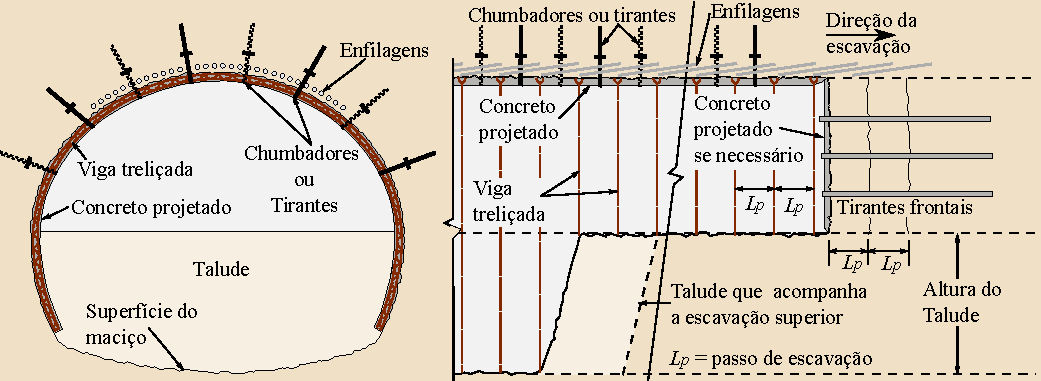
\includegraphics[scale = 0.85]{0312-ilustracao de alguns elementos de presuporte e revestimento.pdf}
	\end{center}
	\caption{\label{ilustracao_elementos_suporte}Ilustração de alguns elementos de pré-suporte e revestimento (adaptado de: \citeonline[p. 9-14]{FederalHighwayAdministration2009})}
\end{figure}

Como este trabalho está delimitado às leis constitutivas do maciço, não foi abordada a diferenciação entre o revestimento primário e secundário. Além do mais, nos modelos desenvolvidos, o revestimento consiste de um material homogêneo, isotrópico e de espessura constante. E a escavação é feita a seção plena, plana e vertical.


